\documentclass[a4paper,12pt,twoside]{article}
\usepackage{rhreport}

\title{Aerial Riparian Solid Waste Mapping}
\author{OpenMap Development Tanzania}

This report was prepared by Glory Emanuel, Immaculate Mwanja, Aaron Eubank, Bornlove Ntikha, Iddy Chazua, Hawa Adinani, Innocent Maholi, Ivan Gayton, William Evans

\date{July 2019}

\begin{document}

\maketitle

\newpage
\tableofcontents

\newpage
\section{Executive Summary}
\begin{multicols}{2}
HOT is an international NGO dedicated to humanitarian action and community development through open mapping. We work together to map data which revolutionises disaster management, reduces risks, and contributes to the achievement of the Sustainable Development Goals.
HOT develops open source apps and tools for collaborative mapping and geospatial data collection. Our tools are free for all to use and leveraged by partners such as Red Cross societies, Médecins Sans Frontières (MSF), UN agencies and programmes, government agencies, and local NGOs and communities.
OMDTZ.

\end{multicols}

\section{Introduction}

Several drone flights were to be  conducted along five major rivers of Dar es Salaam including  Msimbazi, Mpiji, Tegeta, Kizinga and Mzinga rivers, spanning 60 linear kilometers of waterways of Dar es Salaam’s critical water arteries. Msimbazi river was not mapped since it  was  already mapped by World bank. The drone flights provided a digital photographic mark-up of the current status of Dar es Salaam’s waterways.   
Drone flights enable studying any aggregations of waste/informal dumps that are on the banks of the waterways within fifty metres of its bank on either side.Such data is presented as three-dimensional imagery of waste aggregations, further assisting the study team to estimate rough waste volumes.

Drone flights consistently track and record spatial data relating to their own trips and correspond the GIS data with a set of other socio-political and economic indicators, to ease further analysis. This includes:   

\begin{itemize}
    \item The corresponding political division i.e. subward, ward and municipal boundaries—drone flight spatial data overlaid existing socio-political spatial data indicating, via simple desktop analysis, the political constituency that governs each spatial area the drone covers. This allows users to correspond with an informal/illegal dump with the relevant political office that governs the area.
    \item The corresponding density of the geography they are flown over i.e. buildings per sq km/population per sq km via census data. 
\end{itemize}

Drone flights for data collection were conducted within 44 calendar days from 5th April to 18th May 2019, contingent  to the Tanzania Civil Aviation Authority (TCAA) and Ministry of Defence permissions and suitable weather. All technical personnel and equipment required for this assignment are present in Dar es Salaam (site location). 

OMDTZ  combined drone flights and the existing spatial data to conduct a rapid desktop analysis of planned residential and commercial zoning and transport economics as they relate to solid waste management services.

Specifically, spatial analysis allowed the team to quickly present:
\begin{itemize}
    \item Any building or point on a map within the political boundaries of Dar es Salaam that are defined as planned or unplanned.
    \item The complexity of transport from any building in Dar es Salaam to Pugu Kinyamwezi dump site---accounting for two-axle vehicle access, road surface and type, distance and time. 
\end{itemize}
    
Datasets provided audiences with vital data on the inequality of solid waste management infrastructure by geography, as well as providing service providers and government with valuable data on what types of transport modes can be employed to service residents and businesses in planned and unplanned geographies of the city.  

Thereafter, OpenDataKit (ODK) Collect,Kobo Toolbox & QGIS trainings were provided to Nipe Fagio staff. OMDTZ provided an in-depth training on how to upload, analyze and present visual data relating to waste hotpots, informal dumps and cleaning activities.


\newpage
\section{Objectives}

\lipsum[0-1]

\begin{figure}%[H] % uncomment "[H] to force the image to the middle of the page
    \centering
    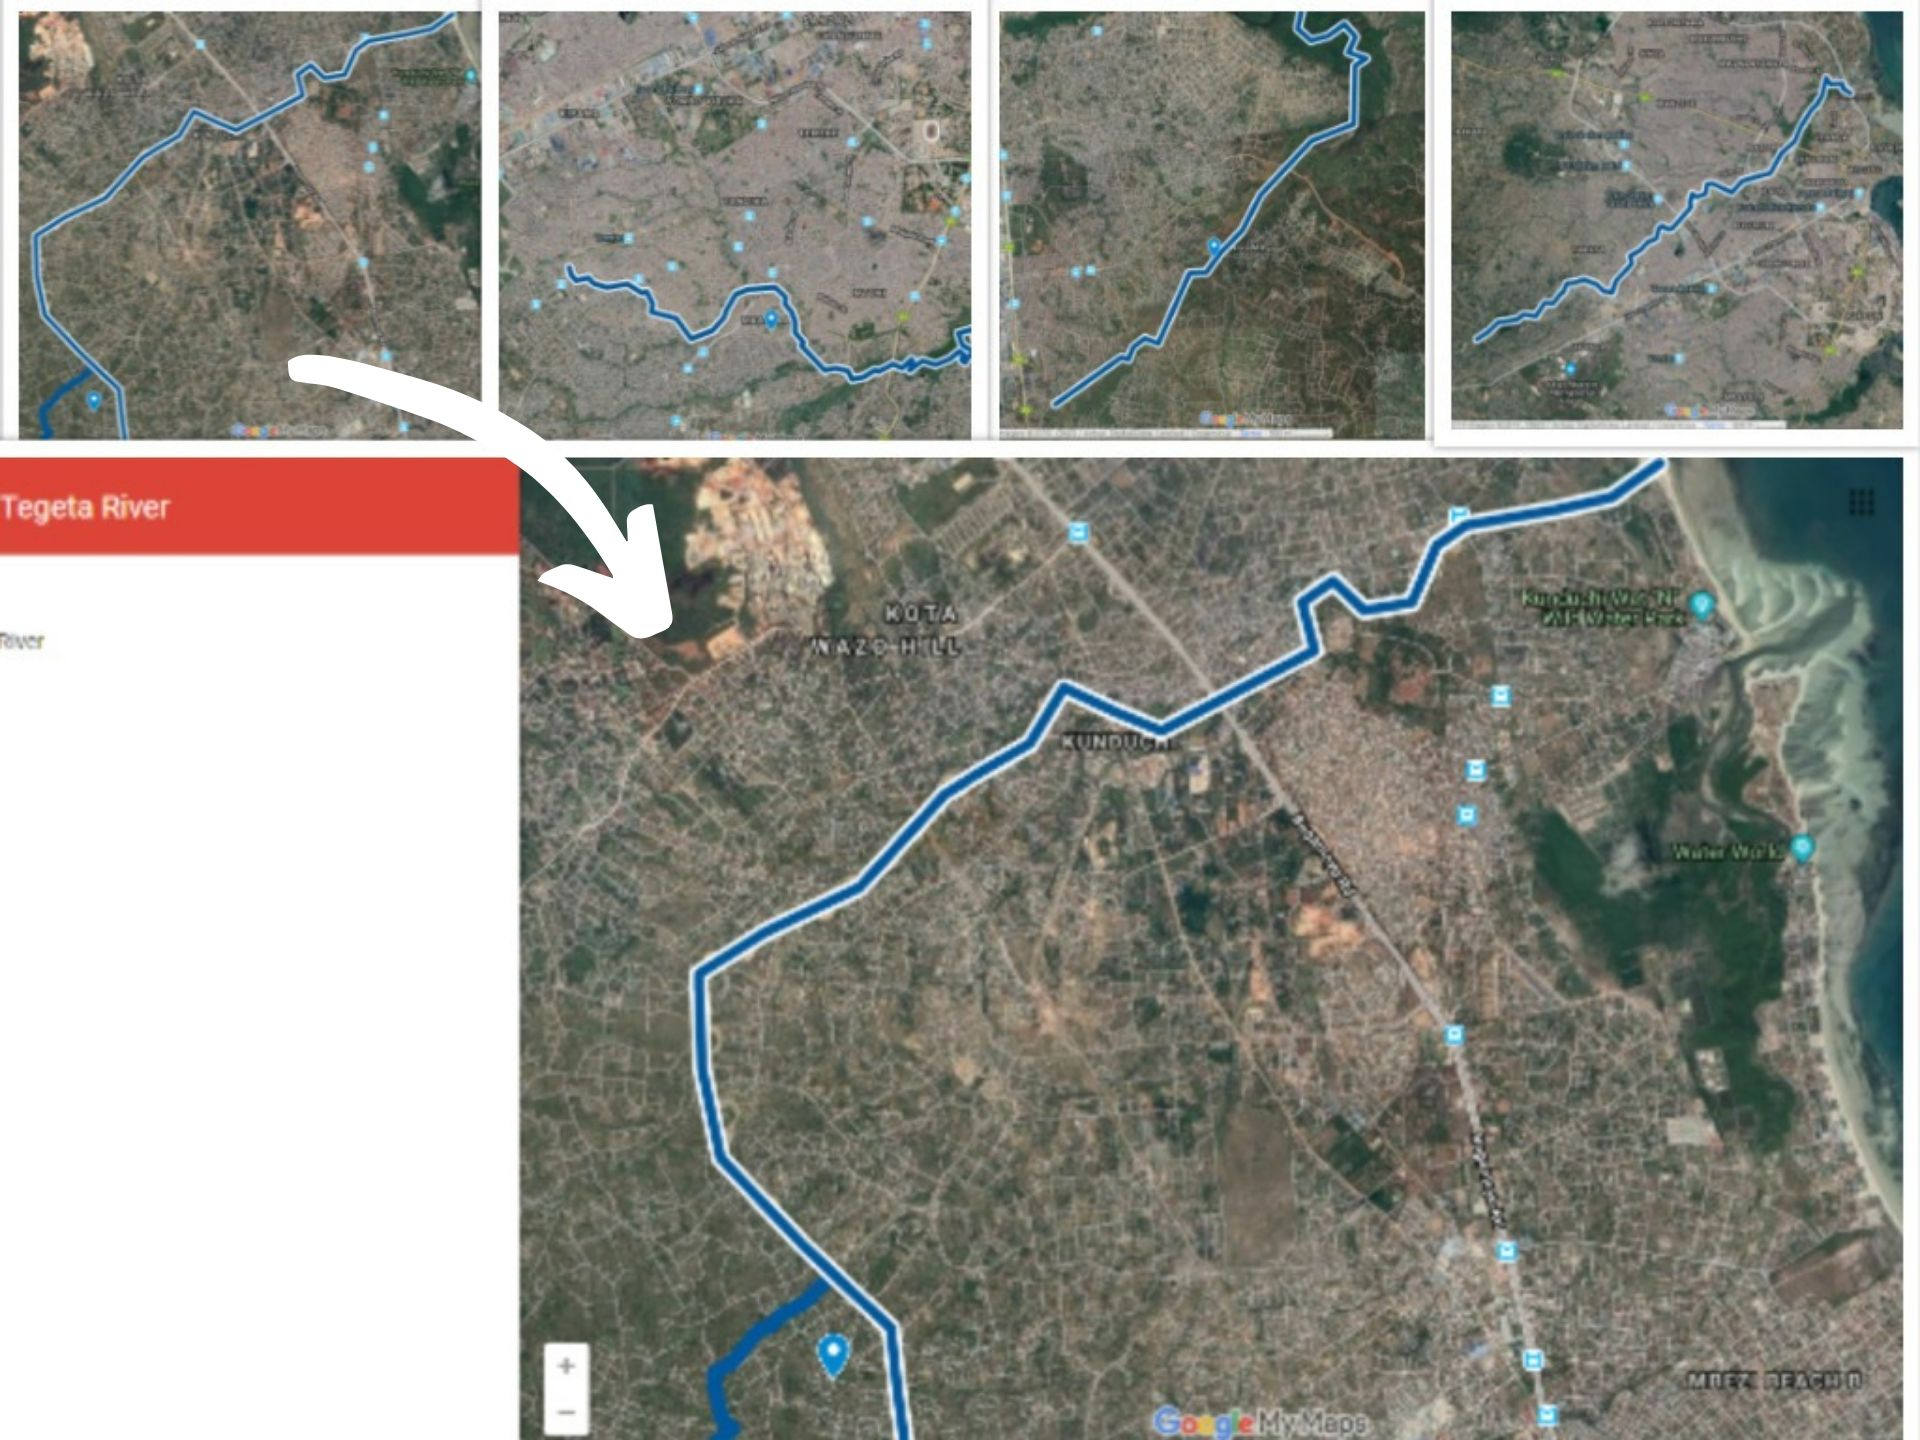
\includegraphics[width=0.8\textwidth]{images/image14.jpg}
    \caption{Screenshot showing missions plans of river mapping}
\end{figure}


\begin{multicols}{2}

\lipsum[0-5]

\end{multicols}

\section{Stakeholders}

\begin{multicols}{2}
\lipsum[0-5]
\end{multicols}

\subsection{Implementing Partners}

\begin{multicols}{2}
\lipsum[0-5]
\end{multicols}

\subsection{Beneficiaries}

\begin{multicols}{2}
\lipsum[0-5]
\end{multicols}

\subsection{Funders}

\begin{multicols}{2}
\lipsum[0-5]
\end{multicols}

\section{Methodology}

\begin{multicols}{2}
\lipsum[0-5]
\end{multicols}

\subsection{Drone Use}

\begin{multicols}{2}
\lipsum[0-5]
\end{multicols}

\subsection{Tools}

\begin{multicols}{2}
\lipsum[0-5]
\end{multicols}

\subsection{UHU Glue for Polystyrene Minor Repair}

\begin{multicols}{2}
\lipsum[0-5]
\end{multicols}

\subsection{MicroSD Cards for Swapping}

\begin{multicols}{2}
\lipsum[0-5]
\end{multicols}

\subsection{Reflector Vest}

\begin{multicols}{2}
\lipsum[0-5]
\end{multicols}

\subsection{Drone Processes}

\begin{multicols}{2}
\lipsum[0-5]
\end{multicols}

\section{Conclusion}

\begin{multicols}{2}
\lipsum[0-5]
\end{multicols}

\subsection{Achievements}

\begin{multicols}{2}
\lipsum[0-5]
\end{multicols}

\subsection{Challenges}

\begin{multicols}{2}
\lipsum[0-5]
\end{multicols}

\subsection{Lessons Learned}

\begin{multicols}{2}
\lipsum[0-5]
\end{multicols}
\subsection{Recommendations}

\begin{multicols}{2}
\lipsum[0-5]
\end{multicols}

\section{Acknowledgements}

\begin{multicols}{2}
\lipsum[0-5]
\end{multicols}

\section{References}

\begin{multicols}{2}
\lipsum[0-5]
\end{multicols}

\section{Training of Nipe Fagio Personnel}

\begin{multicols}{2}
\lipsum[0-5]
\end{multicols}

\subsection{Executive Summary}

\begin{multicols}{2}
\lipsum[0-5]
\end{multicols}

\subsection{Objectives}

\begin{multicols}{2}
\lipsum[0-5]
\end{multicols}

\subsection{OpenDataKit (ODK) Collect Training}

\begin{multicols}{2}
\lipsum[0-5]
\end{multicols}

\subsection{QGIS Training}

\begin{multicols}{2}
\lipsum[0-5]
\end{multicols}

\subsection{Creation of Kobo Toolbox  server for data aggregation}

\begin{multicols}{2}
\lipsum[0-5]
\end{multicols}
	
\subsection{Data Collection Tools}

\begin{multicols}{2}
\lipsum[0-5]
\end{multicols}

\subsection{Map Literacy}

\begin{multicols}{2}
\lipsum[0-5]
\end{multicols}

\subsection{Preparation of Building Clustering and Non-clustering Randomization Manuals}

\begin{multicols}{2}
\lipsum[0-5]
\end{multicols}
\subsection{Waste Management Pilot in Mapped Areas With Nipe Fagio}

\begin{multicols}{2}
\lipsum[0-5]
\end{multicols}

\subsection{Questionnaire}

\begin{multicols}{2}
\lipsum[0-5]
\end{multicols}

\subsection{Data Cleaning using OpenRefine}

\begin{multicols}{2}
\lipsum[0-5]
\end{multicols}

\subsection{Preparation of Interactive Web Map}

\begin{multicols}{2}
\lipsum[0-5]
\end{multicols}

\end{document}

